% Created by tikzDevice version 0.12.3.1 on 2022-05-11 23:32:33
% !TEX encoding = UTF-8 Unicode
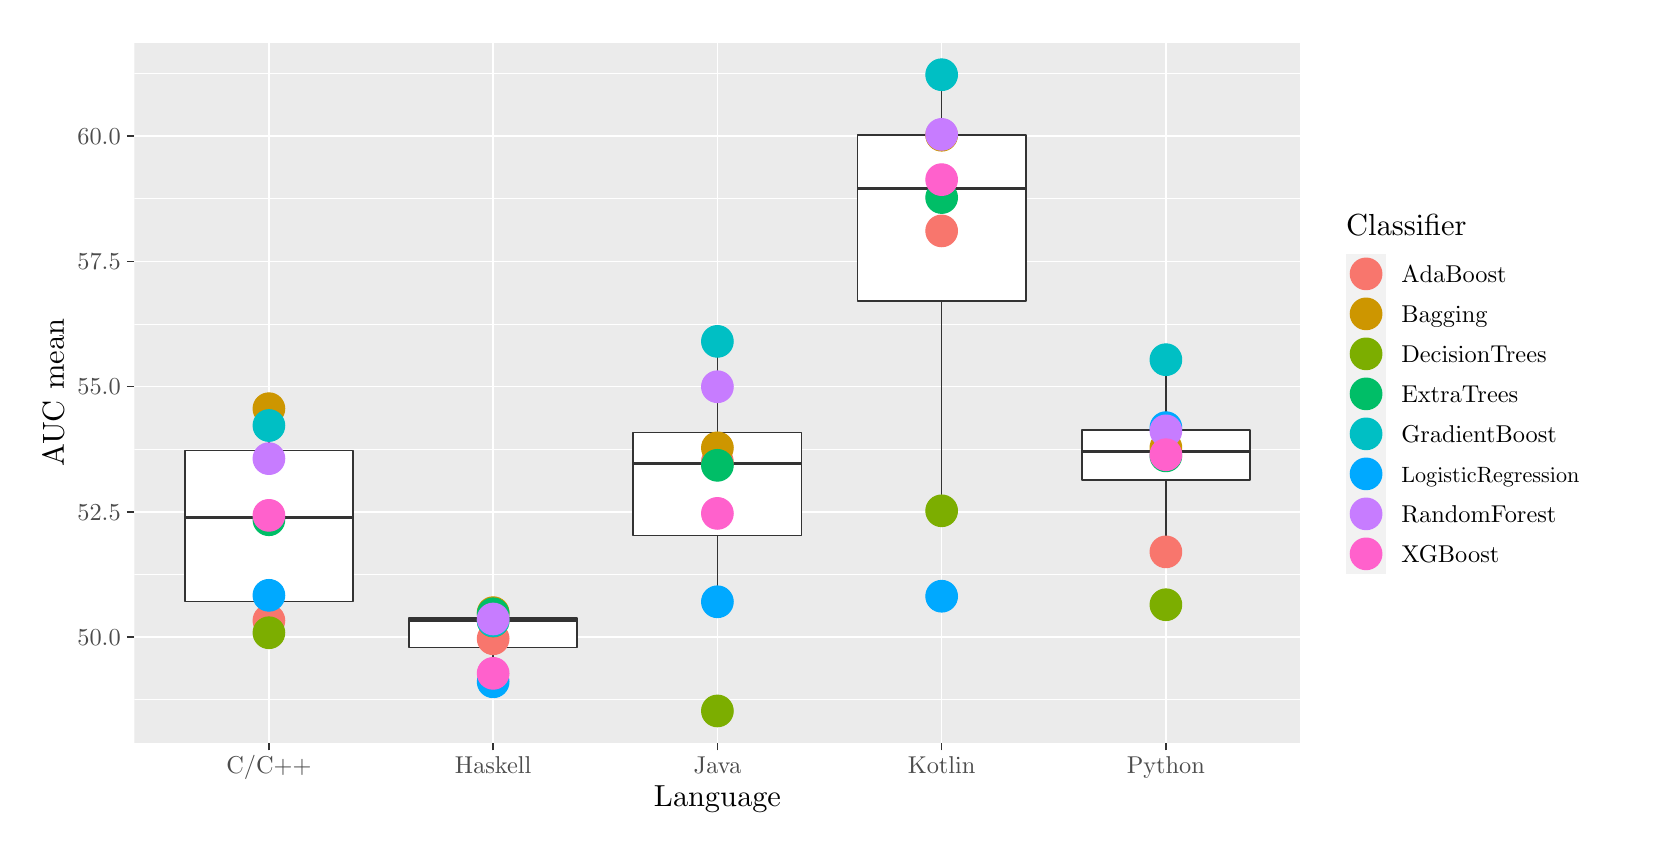
\begin{tikzpicture}[x=1pt,y=1pt]
\definecolor{fillColor}{RGB}{255,255,255}
\path[use as bounding box,fill=fillColor,fill opacity=0.00] (0,0) rectangle (578.16,289.08);
\begin{scope}
\path[clip] (  0.00,  0.00) rectangle (578.16,289.08);
\definecolor{drawColor}{RGB}{255,255,255}
\definecolor{fillColor}{RGB}{255,255,255}

\path[draw=drawColor,line width= 0.6pt,line join=round,line cap=round,fill=fillColor] (  0.00,  0.00) rectangle (578.16,289.08);
\end{scope}
\begin{scope}
\path[clip] ( 38.56, 30.69) rectangle (459.91,283.58);
\definecolor{fillColor}{gray}{0.92}

\path[fill=fillColor] ( 38.56, 30.69) rectangle (459.91,283.58);
\definecolor{drawColor}{RGB}{255,255,255}

\path[draw=drawColor,line width= 0.3pt,line join=round] ( 38.56, 46.34) --
	(459.91, 46.34);

\path[draw=drawColor,line width= 0.3pt,line join=round] ( 38.56, 91.56) --
	(459.91, 91.56);

\path[draw=drawColor,line width= 0.3pt,line join=round] ( 38.56,136.79) --
	(459.91,136.79);

\path[draw=drawColor,line width= 0.3pt,line join=round] ( 38.56,182.01) --
	(459.91,182.01);

\path[draw=drawColor,line width= 0.3pt,line join=round] ( 38.56,227.24) --
	(459.91,227.24);

\path[draw=drawColor,line width= 0.3pt,line join=round] ( 38.56,272.46) --
	(459.91,272.46);

\path[draw=drawColor,line width= 0.6pt,line join=round] ( 38.56, 68.95) --
	(459.91, 68.95);

\path[draw=drawColor,line width= 0.6pt,line join=round] ( 38.56,114.18) --
	(459.91,114.18);

\path[draw=drawColor,line width= 0.6pt,line join=round] ( 38.56,159.40) --
	(459.91,159.40);

\path[draw=drawColor,line width= 0.6pt,line join=round] ( 38.56,204.62) --
	(459.91,204.62);

\path[draw=drawColor,line width= 0.6pt,line join=round] ( 38.56,249.85) --
	(459.91,249.85);

\path[draw=drawColor,line width= 0.6pt,line join=round] ( 87.17, 30.69) --
	( 87.17,283.58);

\path[draw=drawColor,line width= 0.6pt,line join=round] (168.20, 30.69) --
	(168.20,283.58);

\path[draw=drawColor,line width= 0.6pt,line join=round] (249.23, 30.69) --
	(249.23,283.58);

\path[draw=drawColor,line width= 0.6pt,line join=round] (330.26, 30.69) --
	(330.26,283.58);

\path[draw=drawColor,line width= 0.6pt,line join=round] (411.29, 30.69) --
	(411.29,283.58);
\definecolor{drawColor}{gray}{0.20}

\path[draw=drawColor,line width= 0.6pt,line join=round] ( 87.17,136.34) -- ( 87.17,151.40);

\path[draw=drawColor,line width= 0.6pt,line join=round] ( 87.17, 81.68) -- ( 87.17, 70.44);
\definecolor{fillColor}{RGB}{255,255,255}

\path[draw=drawColor,line width= 0.6pt,line join=round,line cap=round,fill=fillColor] ( 56.79,136.34) --
	( 56.79, 81.68) --
	(117.56, 81.68) --
	(117.56,136.34) --
	( 56.79,136.34) --
	cycle;

\path[draw=drawColor,line width= 1.1pt,line join=round] ( 56.79,112.06) -- (117.56,112.06);

\path[draw=drawColor,line width= 0.6pt,line join=round] (168.20, 75.88) -- (168.20, 77.70);

\path[draw=drawColor,line width= 0.6pt,line join=round] (168.20, 65.14) -- (168.20, 52.71);

\path[draw=drawColor,line width= 0.6pt,line join=round,line cap=round,fill=fillColor] (137.82, 75.88) --
	(137.82, 65.14) --
	(198.59, 65.14) --
	(198.59, 75.88) --
	(137.82, 75.88) --
	cycle;

\path[draw=drawColor,line width= 1.1pt,line join=round] (137.82, 74.71) -- (198.59, 74.71);
\definecolor{fillColor}{gray}{0.20}

\path[draw=drawColor,line width= 0.4pt,line join=round,line cap=round,fill=fillColor] (249.23, 42.18) circle (  1.96);

\path[draw=drawColor,line width= 0.6pt,line join=round] (249.23,142.77) -- (249.23,175.72);

\path[draw=drawColor,line width= 0.6pt,line join=round] (249.23,105.58) -- (249.23, 81.63);
\definecolor{fillColor}{RGB}{255,255,255}

\path[draw=drawColor,line width= 0.6pt,line join=round,line cap=round,fill=fillColor] (218.85,142.77) --
	(218.85,105.58) --
	(279.62,105.58) --
	(279.62,142.77) --
	(218.85,142.77) --
	cycle;

\path[draw=drawColor,line width= 1.1pt,line join=round] (218.85,131.59) -- (279.62,131.59);
\definecolor{fillColor}{gray}{0.20}

\path[draw=drawColor,line width= 0.4pt,line join=round,line cap=round,fill=fillColor] (330.26, 83.63) circle (  1.96);

\path[draw=drawColor,line width= 0.6pt,line join=round] (330.26,250.29) -- (330.26,272.08);

\path[draw=drawColor,line width= 0.6pt,line join=round] (330.26,190.35) -- (330.26,114.50);
\definecolor{fillColor}{RGB}{255,255,255}

\path[draw=drawColor,line width= 0.6pt,line join=round,line cap=round,fill=fillColor] (299.87,250.29) --
	(299.87,190.35) --
	(360.65,190.35) --
	(360.65,250.29) --
	(299.87,250.29) --
	cycle;

\path[draw=drawColor,line width= 1.1pt,line join=round] (299.87,230.93) -- (360.65,230.93);
\definecolor{fillColor}{gray}{0.20}

\path[draw=drawColor,line width= 0.4pt,line join=round,line cap=round,fill=fillColor] (411.29, 80.56) circle (  1.96);

\path[draw=drawColor,line width= 0.6pt,line join=round] (411.29,143.68) -- (411.29,169.11);

\path[draw=drawColor,line width= 0.6pt,line join=round] (411.29,125.67) -- (411.29, 99.66);
\definecolor{fillColor}{RGB}{255,255,255}

\path[draw=drawColor,line width= 0.6pt,line join=round,line cap=round,fill=fillColor] (380.90,143.68) --
	(380.90,125.67) --
	(441.68,125.67) --
	(441.68,143.68) --
	(380.90,143.68) --
	cycle;

\path[draw=drawColor,line width= 1.1pt,line join=round] (380.90,136.05) -- (441.68,136.05);
\definecolor{drawColor}{RGB}{248,118,109}
\definecolor{fillColor}{RGB}{248,118,109}

\path[draw=drawColor,line width= 0.4pt,line join=round,line cap=round,fill=fillColor] ( 87.17, 74.84) circle (  5.71);
\definecolor{drawColor}{RGB}{205,150,0}
\definecolor{fillColor}{RGB}{205,150,0}

\path[draw=drawColor,line width= 0.4pt,line join=round,line cap=round,fill=fillColor] ( 87.17,151.40) circle (  5.71);
\definecolor{drawColor}{RGB}{124,174,0}
\definecolor{fillColor}{RGB}{124,174,0}

\path[draw=drawColor,line width= 0.4pt,line join=round,line cap=round,fill=fillColor] ( 87.17, 70.44) circle (  5.71);
\definecolor{drawColor}{RGB}{0,190,103}
\definecolor{fillColor}{RGB}{0,190,103}

\path[draw=drawColor,line width= 0.4pt,line join=round,line cap=round,fill=fillColor] ( 87.17,111.27) circle (  5.71);
\definecolor{drawColor}{RGB}{0,191,196}
\definecolor{fillColor}{RGB}{0,191,196}

\path[draw=drawColor,line width= 0.4pt,line join=round,line cap=round,fill=fillColor] ( 87.17,145.31) circle (  5.71);
\definecolor{drawColor}{RGB}{0,169,255}
\definecolor{fillColor}{RGB}{0,169,255}

\path[draw=drawColor,line width= 0.4pt,line join=round,line cap=round,fill=fillColor] ( 87.17, 83.96) circle (  5.71);
\definecolor{drawColor}{RGB}{199,124,255}
\definecolor{fillColor}{RGB}{199,124,255}

\path[draw=drawColor,line width= 0.4pt,line join=round,line cap=round,fill=fillColor] ( 87.17,133.35) circle (  5.71);
\definecolor{drawColor}{RGB}{255,97,204}
\definecolor{fillColor}{RGB}{255,97,204}

\path[draw=drawColor,line width= 0.4pt,line join=round,line cap=round,fill=fillColor] ( 87.17,112.85) circle (  5.71);
\definecolor{drawColor}{RGB}{248,118,109}
\definecolor{fillColor}{RGB}{248,118,109}

\path[draw=drawColor,line width= 0.4pt,line join=round,line cap=round,fill=fillColor] (168.20, 68.27) circle (  5.71);
\definecolor{drawColor}{RGB}{205,150,0}
\definecolor{fillColor}{RGB}{205,150,0}

\path[draw=drawColor,line width= 0.4pt,line join=round,line cap=round,fill=fillColor] (168.20, 77.70) circle (  5.71);
\definecolor{drawColor}{RGB}{124,174,0}
\definecolor{fillColor}{RGB}{124,174,0}

\path[draw=drawColor,line width= 0.4pt,line join=round,line cap=round,fill=fillColor] (168.20, 74.68) circle (  5.71);
\definecolor{drawColor}{RGB}{0,190,103}
\definecolor{fillColor}{RGB}{0,190,103}

\path[draw=drawColor,line width= 0.4pt,line join=round,line cap=round,fill=fillColor] (168.20, 77.29) circle (  5.71);
\definecolor{drawColor}{RGB}{0,191,196}
\definecolor{fillColor}{RGB}{0,191,196}

\path[draw=drawColor,line width= 0.4pt,line join=round,line cap=round,fill=fillColor] (168.20, 74.74) circle (  5.71);
\definecolor{drawColor}{RGB}{0,169,255}
\definecolor{fillColor}{RGB}{0,169,255}

\path[draw=drawColor,line width= 0.4pt,line join=round,line cap=round,fill=fillColor] (168.20, 52.71) circle (  5.71);
\definecolor{drawColor}{RGB}{199,124,255}
\definecolor{fillColor}{RGB}{199,124,255}

\path[draw=drawColor,line width= 0.4pt,line join=round,line cap=round,fill=fillColor] (168.20, 75.41) circle (  5.71);
\definecolor{drawColor}{RGB}{255,97,204}
\definecolor{fillColor}{RGB}{255,97,204}

\path[draw=drawColor,line width= 0.4pt,line join=round,line cap=round,fill=fillColor] (168.20, 55.76) circle (  5.71);
\definecolor{drawColor}{RGB}{248,118,109}
\definecolor{fillColor}{RGB}{248,118,109}

\path[draw=drawColor,line width= 0.4pt,line join=round,line cap=round,fill=fillColor] (249.23,132.25) circle (  5.71);
\definecolor{drawColor}{RGB}{205,150,0}
\definecolor{fillColor}{RGB}{205,150,0}

\path[draw=drawColor,line width= 0.4pt,line join=round,line cap=round,fill=fillColor] (249.23,137.25) circle (  5.71);
\definecolor{drawColor}{RGB}{124,174,0}
\definecolor{fillColor}{RGB}{124,174,0}

\path[draw=drawColor,line width= 0.4pt,line join=round,line cap=round,fill=fillColor] (249.23, 42.18) circle (  5.71);
\definecolor{drawColor}{RGB}{0,190,103}
\definecolor{fillColor}{RGB}{0,190,103}

\path[draw=drawColor,line width= 0.4pt,line join=round,line cap=round,fill=fillColor] (249.23,130.93) circle (  5.71);
\definecolor{drawColor}{RGB}{0,191,196}
\definecolor{fillColor}{RGB}{0,191,196}

\path[draw=drawColor,line width= 0.4pt,line join=round,line cap=round,fill=fillColor] (249.23,175.72) circle (  5.71);
\definecolor{drawColor}{RGB}{0,169,255}
\definecolor{fillColor}{RGB}{0,169,255}

\path[draw=drawColor,line width= 0.4pt,line join=round,line cap=round,fill=fillColor] (249.23, 81.63) circle (  5.71);
\definecolor{drawColor}{RGB}{199,124,255}
\definecolor{fillColor}{RGB}{199,124,255}

\path[draw=drawColor,line width= 0.4pt,line join=round,line cap=round,fill=fillColor] (249.23,159.33) circle (  5.71);
\definecolor{drawColor}{RGB}{255,97,204}
\definecolor{fillColor}{RGB}{255,97,204}

\path[draw=drawColor,line width= 0.4pt,line join=round,line cap=round,fill=fillColor] (249.23,113.56) circle (  5.71);
\definecolor{drawColor}{RGB}{248,118,109}
\definecolor{fillColor}{RGB}{248,118,109}

\path[draw=drawColor,line width= 0.4pt,line join=round,line cap=round,fill=fillColor] (330.26,215.64) circle (  5.71);
\definecolor{drawColor}{RGB}{205,150,0}
\definecolor{fillColor}{RGB}{205,150,0}

\path[draw=drawColor,line width= 0.4pt,line join=round,line cap=round,fill=fillColor] (330.26,250.21) circle (  5.71);
\definecolor{drawColor}{RGB}{124,174,0}
\definecolor{fillColor}{RGB}{124,174,0}

\path[draw=drawColor,line width= 0.4pt,line join=round,line cap=round,fill=fillColor] (330.26,114.50) circle (  5.71);
\definecolor{drawColor}{RGB}{0,190,103}
\definecolor{fillColor}{RGB}{0,190,103}

\path[draw=drawColor,line width= 0.4pt,line join=round,line cap=round,fill=fillColor] (330.26,227.69) circle (  5.71);
\definecolor{drawColor}{RGB}{0,191,196}
\definecolor{fillColor}{RGB}{0,191,196}

\path[draw=drawColor,line width= 0.4pt,line join=round,line cap=round,fill=fillColor] (330.26,272.08) circle (  5.71);
\definecolor{drawColor}{RGB}{0,169,255}
\definecolor{fillColor}{RGB}{0,169,255}

\path[draw=drawColor,line width= 0.4pt,line join=round,line cap=round,fill=fillColor] (330.26, 83.63) circle (  5.71);
\definecolor{drawColor}{RGB}{199,124,255}
\definecolor{fillColor}{RGB}{199,124,255}

\path[draw=drawColor,line width= 0.4pt,line join=round,line cap=round,fill=fillColor] (330.26,250.52) circle (  5.71);
\definecolor{drawColor}{RGB}{255,97,204}
\definecolor{fillColor}{RGB}{255,97,204}

\path[draw=drawColor,line width= 0.4pt,line join=round,line cap=round,fill=fillColor] (330.26,234.17) circle (  5.71);
\definecolor{drawColor}{RGB}{248,118,109}
\definecolor{fillColor}{RGB}{248,118,109}

\path[draw=drawColor,line width= 0.4pt,line join=round,line cap=round,fill=fillColor] (411.29, 99.66) circle (  5.71);
\definecolor{drawColor}{RGB}{205,150,0}
\definecolor{fillColor}{RGB}{205,150,0}

\path[draw=drawColor,line width= 0.4pt,line join=round,line cap=round,fill=fillColor] (411.29,137.33) circle (  5.71);
\definecolor{drawColor}{RGB}{124,174,0}
\definecolor{fillColor}{RGB}{124,174,0}

\path[draw=drawColor,line width= 0.4pt,line join=round,line cap=round,fill=fillColor] (411.29, 80.56) circle (  5.71);
\definecolor{drawColor}{RGB}{0,190,103}
\definecolor{fillColor}{RGB}{0,190,103}

\path[draw=drawColor,line width= 0.4pt,line join=round,line cap=round,fill=fillColor] (411.29,134.34) circle (  5.71);
\definecolor{drawColor}{RGB}{0,191,196}
\definecolor{fillColor}{RGB}{0,191,196}

\path[draw=drawColor,line width= 0.4pt,line join=round,line cap=round,fill=fillColor] (411.29,169.11) circle (  5.71);
\definecolor{drawColor}{RGB}{0,169,255}
\definecolor{fillColor}{RGB}{0,169,255}

\path[draw=drawColor,line width= 0.4pt,line join=round,line cap=round,fill=fillColor] (411.29,144.55) circle (  5.71);
\definecolor{drawColor}{RGB}{199,124,255}
\definecolor{fillColor}{RGB}{199,124,255}

\path[draw=drawColor,line width= 0.4pt,line join=round,line cap=round,fill=fillColor] (411.29,143.39) circle (  5.71);
\definecolor{drawColor}{RGB}{255,97,204}
\definecolor{fillColor}{RGB}{255,97,204}

\path[draw=drawColor,line width= 0.4pt,line join=round,line cap=round,fill=fillColor] (411.29,134.77) circle (  5.71);
\end{scope}
\begin{scope}
\path[clip] (  0.00,  0.00) rectangle (578.16,289.08);
\definecolor{drawColor}{gray}{0.30}

\node[text=drawColor,anchor=base east,inner sep=0pt, outer sep=0pt, scale=  0.88] at ( 33.61, 65.92) {50.0};

\node[text=drawColor,anchor=base east,inner sep=0pt, outer sep=0pt, scale=  0.88] at ( 33.61,111.15) {52.5};

\node[text=drawColor,anchor=base east,inner sep=0pt, outer sep=0pt, scale=  0.88] at ( 33.61,156.37) {55.0};

\node[text=drawColor,anchor=base east,inner sep=0pt, outer sep=0pt, scale=  0.88] at ( 33.61,201.59) {57.5};

\node[text=drawColor,anchor=base east,inner sep=0pt, outer sep=0pt, scale=  0.88] at ( 33.61,246.82) {60.0};
\end{scope}
\begin{scope}
\path[clip] (  0.00,  0.00) rectangle (578.16,289.08);
\definecolor{drawColor}{gray}{0.20}

\path[draw=drawColor,line width= 0.6pt,line join=round] ( 35.81, 68.95) --
	( 38.56, 68.95);

\path[draw=drawColor,line width= 0.6pt,line join=round] ( 35.81,114.18) --
	( 38.56,114.18);

\path[draw=drawColor,line width= 0.6pt,line join=round] ( 35.81,159.40) --
	( 38.56,159.40);

\path[draw=drawColor,line width= 0.6pt,line join=round] ( 35.81,204.62) --
	( 38.56,204.62);

\path[draw=drawColor,line width= 0.6pt,line join=round] ( 35.81,249.85) --
	( 38.56,249.85);
\end{scope}
\begin{scope}
\path[clip] (  0.00,  0.00) rectangle (578.16,289.08);
\definecolor{drawColor}{gray}{0.20}

\path[draw=drawColor,line width= 0.6pt,line join=round] ( 87.17, 27.94) --
	( 87.17, 30.69);

\path[draw=drawColor,line width= 0.6pt,line join=round] (168.20, 27.94) --
	(168.20, 30.69);

\path[draw=drawColor,line width= 0.6pt,line join=round] (249.23, 27.94) --
	(249.23, 30.69);

\path[draw=drawColor,line width= 0.6pt,line join=round] (330.26, 27.94) --
	(330.26, 30.69);

\path[draw=drawColor,line width= 0.6pt,line join=round] (411.29, 27.94) --
	(411.29, 30.69);
\end{scope}
\begin{scope}
\path[clip] (  0.00,  0.00) rectangle (578.16,289.08);
\definecolor{drawColor}{gray}{0.30}

\node[text=drawColor,anchor=base,inner sep=0pt, outer sep=0pt, scale=  0.88] at ( 87.17, 19.68) {C/C++};

\node[text=drawColor,anchor=base,inner sep=0pt, outer sep=0pt, scale=  0.88] at (168.20, 19.68) {Haskell};

\node[text=drawColor,anchor=base,inner sep=0pt, outer sep=0pt, scale=  0.88] at (249.23, 19.68) {Java};

\node[text=drawColor,anchor=base,inner sep=0pt, outer sep=0pt, scale=  0.88] at (330.26, 19.68) {Kotlin};

\node[text=drawColor,anchor=base,inner sep=0pt, outer sep=0pt, scale=  0.88] at (411.29, 19.68) {Python};
\end{scope}
\begin{scope}
\path[clip] (  0.00,  0.00) rectangle (578.16,289.08);
\definecolor{drawColor}{RGB}{0,0,0}

\node[text=drawColor,anchor=base,inner sep=0pt, outer sep=0pt, scale=  1.10] at (249.23,  7.64) {Language};
\end{scope}
\begin{scope}
\path[clip] (  0.00,  0.00) rectangle (578.16,289.08);
\definecolor{drawColor}{RGB}{0,0,0}

\node[text=drawColor,rotate= 90.00,anchor=base,inner sep=0pt, outer sep=0pt, scale=  1.10] at ( 13.08,157.13) {AUC mean};
\end{scope}
\begin{scope}
\path[clip] (  0.00,  0.00) rectangle (578.16,289.08);
\definecolor{fillColor}{RGB}{255,255,255}

\path[fill=fillColor] (470.91, 86.21) rectangle (572.66,228.06);
\end{scope}
\begin{scope}
\path[clip] (  0.00,  0.00) rectangle (578.16,289.08);
\definecolor{drawColor}{RGB}{0,0,0}

\node[text=drawColor,anchor=base west,inner sep=0pt, outer sep=0pt, scale=  1.10] at (476.41,213.91) {Classifier};
\end{scope}
\begin{scope}
\path[clip] (  0.00,  0.00) rectangle (578.16,289.08);
\definecolor{fillColor}{gray}{0.95}

\path[fill=fillColor] (476.41,192.89) rectangle (490.86,207.34);
\end{scope}
\begin{scope}
\path[clip] (  0.00,  0.00) rectangle (578.16,289.08);
\definecolor{drawColor}{RGB}{248,118,109}
\definecolor{fillColor}{RGB}{248,118,109}

\path[draw=drawColor,line width= 0.4pt,line join=round,line cap=round,fill=fillColor] (483.63,200.11) circle (  5.71);
\end{scope}
\begin{scope}
\path[clip] (  0.00,  0.00) rectangle (578.16,289.08);
\definecolor{fillColor}{gray}{0.95}

\path[fill=fillColor] (476.41,178.43) rectangle (490.86,192.89);
\end{scope}
\begin{scope}
\path[clip] (  0.00,  0.00) rectangle (578.16,289.08);
\definecolor{drawColor}{RGB}{205,150,0}
\definecolor{fillColor}{RGB}{205,150,0}

\path[draw=drawColor,line width= 0.4pt,line join=round,line cap=round,fill=fillColor] (483.63,185.66) circle (  5.71);
\end{scope}
\begin{scope}
\path[clip] (  0.00,  0.00) rectangle (578.16,289.08);
\definecolor{fillColor}{gray}{0.95}

\path[fill=fillColor] (476.41,163.98) rectangle (490.86,178.43);
\end{scope}
\begin{scope}
\path[clip] (  0.00,  0.00) rectangle (578.16,289.08);
\definecolor{drawColor}{RGB}{124,174,0}
\definecolor{fillColor}{RGB}{124,174,0}

\path[draw=drawColor,line width= 0.4pt,line join=round,line cap=round,fill=fillColor] (483.63,171.21) circle (  5.71);
\end{scope}
\begin{scope}
\path[clip] (  0.00,  0.00) rectangle (578.16,289.08);
\definecolor{fillColor}{gray}{0.95}

\path[fill=fillColor] (476.41,149.53) rectangle (490.86,163.98);
\end{scope}
\begin{scope}
\path[clip] (  0.00,  0.00) rectangle (578.16,289.08);
\definecolor{drawColor}{RGB}{0,190,103}
\definecolor{fillColor}{RGB}{0,190,103}

\path[draw=drawColor,line width= 0.4pt,line join=round,line cap=round,fill=fillColor] (483.63,156.75) circle (  5.71);
\end{scope}
\begin{scope}
\path[clip] (  0.00,  0.00) rectangle (578.16,289.08);
\definecolor{fillColor}{gray}{0.95}

\path[fill=fillColor] (476.41,135.07) rectangle (490.86,149.53);
\end{scope}
\begin{scope}
\path[clip] (  0.00,  0.00) rectangle (578.16,289.08);
\definecolor{drawColor}{RGB}{0,191,196}
\definecolor{fillColor}{RGB}{0,191,196}

\path[draw=drawColor,line width= 0.4pt,line join=round,line cap=round,fill=fillColor] (483.63,142.30) circle (  5.71);
\end{scope}
\begin{scope}
\path[clip] (  0.00,  0.00) rectangle (578.16,289.08);
\definecolor{fillColor}{gray}{0.95}

\path[fill=fillColor] (476.41,120.62) rectangle (490.86,135.07);
\end{scope}
\begin{scope}
\path[clip] (  0.00,  0.00) rectangle (578.16,289.08);
\definecolor{drawColor}{RGB}{0,169,255}
\definecolor{fillColor}{RGB}{0,169,255}

\path[draw=drawColor,line width= 0.4pt,line join=round,line cap=round,fill=fillColor] (483.63,127.84) circle (  5.71);
\end{scope}
\begin{scope}
\path[clip] (  0.00,  0.00) rectangle (578.16,289.08);
\definecolor{fillColor}{gray}{0.95}

\path[fill=fillColor] (476.41,106.16) rectangle (490.86,120.62);
\end{scope}
\begin{scope}
\path[clip] (  0.00,  0.00) rectangle (578.16,289.08);
\definecolor{drawColor}{RGB}{199,124,255}
\definecolor{fillColor}{RGB}{199,124,255}

\path[draw=drawColor,line width= 0.4pt,line join=round,line cap=round,fill=fillColor] (483.63,113.39) circle (  5.71);
\end{scope}
\begin{scope}
\path[clip] (  0.00,  0.00) rectangle (578.16,289.08);
\definecolor{fillColor}{gray}{0.95}

\path[fill=fillColor] (476.41, 91.71) rectangle (490.86,106.16);
\end{scope}
\begin{scope}
\path[clip] (  0.00,  0.00) rectangle (578.16,289.08);
\definecolor{drawColor}{RGB}{255,97,204}
\definecolor{fillColor}{RGB}{255,97,204}

\path[draw=drawColor,line width= 0.4pt,line join=round,line cap=round,fill=fillColor] (483.63, 98.94) circle (  5.71);
\end{scope}
\begin{scope}
\path[clip] (  0.00,  0.00) rectangle (578.16,289.08);
\definecolor{drawColor}{RGB}{0,0,0}

\node[text=drawColor,anchor=base west,inner sep=0pt, outer sep=0pt, scale=  0.88] at (496.36,197.08) {AdaBoost};
\end{scope}
\begin{scope}
\path[clip] (  0.00,  0.00) rectangle (578.16,289.08);
\definecolor{drawColor}{RGB}{0,0,0}

\node[text=drawColor,anchor=base west,inner sep=0pt, outer sep=0pt, scale=  0.88] at (496.36,182.63) {Bagging};
\end{scope}
\begin{scope}
\path[clip] (  0.00,  0.00) rectangle (578.16,289.08);
\definecolor{drawColor}{RGB}{0,0,0}

\node[text=drawColor,anchor=base west,inner sep=0pt, outer sep=0pt, scale=  0.88] at (496.36,168.18) {DecisionTrees};
\end{scope}
\begin{scope}
\path[clip] (  0.00,  0.00) rectangle (578.16,289.08);
\definecolor{drawColor}{RGB}{0,0,0}

\node[text=drawColor,anchor=base west,inner sep=0pt, outer sep=0pt, scale=  0.88] at (496.36,153.72) {ExtraTrees};
\end{scope}
\begin{scope}
\path[clip] (  0.00,  0.00) rectangle (578.16,289.08);
\definecolor{drawColor}{RGB}{0,0,0}

\node[text=drawColor,anchor=base west,inner sep=0pt, outer sep=0pt, scale=  0.88] at (496.36,139.27) {GradientBoost};
\end{scope}
\begin{scope}
\path[clip] (  0.00,  0.00) rectangle (578.16,289.08);
\definecolor{drawColor}{RGB}{0,0,0}

\node[text=drawColor,anchor=base west,inner sep=0pt, outer sep=0pt, scale=  0.80] at (496.36,124.81) {LogisticRegression};
\end{scope}
\begin{scope}
\path[clip] (  0.00,  0.00) rectangle (578.16,289.08);
\definecolor{drawColor}{RGB}{0,0,0}

\node[text=drawColor,anchor=base west,inner sep=0pt, outer sep=0pt, scale=  0.88] at (496.36,110.36) {RandomForest};
\end{scope}
\begin{scope}
\path[clip] (  0.00,  0.00) rectangle (578.16,289.08);
\definecolor{drawColor}{RGB}{0,0,0}

\node[text=drawColor,anchor=base west,inner sep=0pt, outer sep=0pt, scale=  0.88] at (496.36, 95.91) {XGBoost};
\end{scope}
\end{tikzpicture}
